%% Please fill in your name and collaboration statement here.
\newcommand{\studentName}{**FILL IN YOUR NAME HERE**}
\newcommand{\collaborationStatement}{**FILL IN YOUR COLLABORATION STATEMENT HERE \\ (See the syllabus for information)**}


%%%%%%%%%%%%%%%%%%%%%%%%%%%%%%%%%%%%%%%%%%%%%%%
\documentclass[solution, letterpaper]{cs20inclass}
\usepackage{enumerate}
\usepackage{tikz}
\usepackage{pgf}
\usepackage{tikz}
\usepackage{hyperref}
\begin{document}
\header{1}{Monday, January 25, 2016}

\noindent Author: Hannah Blumberg% \\

\paragraph*{Check-In Question}
\begin{enumerate}

\item
You awake in your tent in pitch darkness and need to get dressed. You know that your knapsack contains white, brown, blue, and black socks. Use the pigeonhole principle (even if you have not known it by that name) to determine the minimum number of socks that you must carry to the nearby campfire in order to be sure of having a pair with matching colors.
\begin{enumerate}
\item 5
\item 6
\item 7
\item 8
\end{enumerate}

\textbf{Solution:} (a)

$4\text{ sock colors } + 1 = 5$

\end{enumerate}

\problem

The key step for each problem is to identify the appropriate ``pigeons'' and ``pigeonholes.''

\subproblem Choose any five points inside the unit square. Prove that there is at least one pair for which the distance between the points is less than $\frac{1}{\sqrt{2}}$. Hint: Split the square into equal-sized regions.

\subproblem (BONUS) Show in the case of the $5\times5$ grid problem done in the minilecture that some square winds up empty.

\begin{solution}
  \subsolution 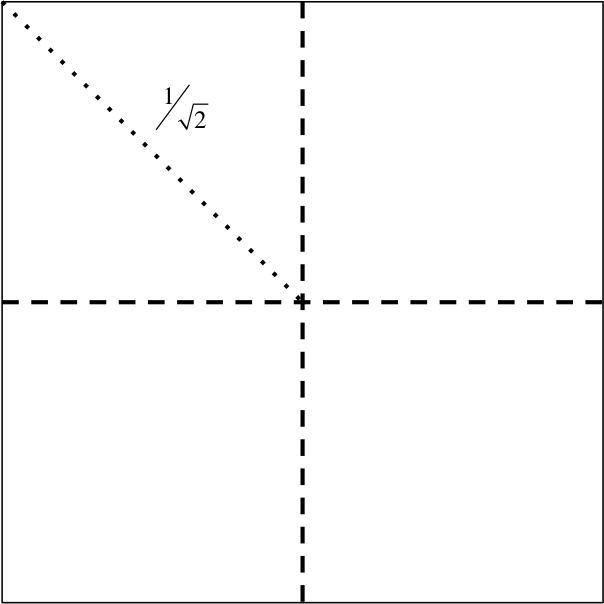
\includegraphics[width=6cm]{01-1}

If the unit square is divided into 4 quarters, then within each quarter, each pair of dots is at most $\frac{1}{\sqrt{2}}$ units away. (Calculated using the Pythagorean theorem.)

Let the 5 points be the pigeons and let the 4 quarters be the pigeonholes. By the pigeonhole principle, at least 1 quarter will have at least 2 points. As a result, there must be at least 1 pair of points for which the distance between the points is less than $\frac{1}{\sqrt{2}}$.
  \\
  \subsolution 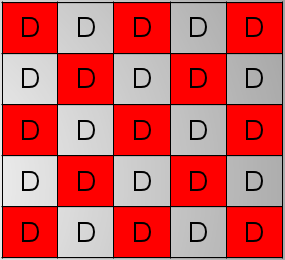
\includegraphics[width=6cm]{01-2}

As we saw in the minilecture, birds in red squares can only move to gray squares and birds in gray squares can only move to red squares.

Let the 13 red squares be the pigeons and let the 12 birds on the gray squares be the pigeonholes. We will ``assign'' each of the 12 birds a red square to which they will move. By the pigeonhole principle, at least 1 bird will be assigned at least 2 red squares. Since a bird can only be in 1 square at a time, at least 1 square will be left empty.
\end{solution}

\end{document}
